% ============================================================================
%  AI-Driven Educational Analytics System — Technical Project Report
%  Intelligent Exam-Question Difficulty Prediction using Feature Engineering,
%  Logistic Regression, Agentic Workflows & Retrieval-Augmented Generation.
% ============================================================================

\documentclass[12pt, a4paper, twoside]{article}

% --- Packages ---------------------------------------------------------------
\usepackage[utf8]{inputenc}
\usepackage[T1]{fontenc}
\usepackage{lmodern}
\usepackage[margin=1in]{geometry}
\usepackage{graphicx}
\usepackage{booktabs}
\usepackage{array}
\usepackage{amsmath, amssymb}
\usepackage{xcolor}
\usepackage{hyperref}
\usepackage{enumitem}
\usepackage{caption}
\usepackage{subcaption}
\usepackage{float}
\usepackage{listings}
\usepackage{fancyhdr}
\usepackage{titlesec}
\usepackage{tocloft}
\usepackage{parskip}
\usepackage{multirow}
\usepackage{tabularx}
\usepackage{longtable}
\usepackage{tikz}
\usepackage{algpseudocode}
\usepackage{algorithm}
\usepackage{csquotes}
\usepackage{url}
\usetikzlibrary{shapes.geometric, arrows.meta, positioning, calc, fit,
                backgrounds, decorations.pathreplacing, shadows.blur}

% --- Colour Palette ---------------------------------------------------------
\definecolor{primary}{HTML}{1E293B}
\definecolor{accent}{HTML}{2563EB}
\definecolor{muted}{HTML}{94A3B8}
\definecolor{codebg}{HTML}{F1F5F9}
\definecolor{linkblue}{HTML}{3B82F6}
\definecolor{easygreen}{HTML}{16A34A}
\definecolor{medamber}{HTML}{D97706}
\definecolor{hardred}{HTML}{DC2626}
\definecolor{agentpurple}{HTML}{7C3AED}
\definecolor{ragcyan}{HTML}{0891B2}
\definecolor{sectionrule}{HTML}{CBD5E1}

% --- Hyperref Setup ---------------------------------------------------------
\hypersetup{
    colorlinks  = true,
    linkcolor   = primary,
    urlcolor    = linkblue,
    citecolor   = accent,
    pdftitle    = {AI-Driven Educational Analytics System — Technical Project Report},
    pdfauthor   = {Siddharth Dangi},
    pdfsubject  = {Machine Learning, Agentic AI, RAG, Educational Analytics},
    pdfkeywords = {TF-IDF, Logistic Regression, LangGraph, RAG, FAISS,
                   Gemini, Educational Assessment, Difficulty Prediction},
}

% --- Header / Footer --------------------------------------------------------
\pagestyle{fancy}
\fancyhf{}
\fancyhead[LE,RO]{\small\textcolor{muted}{\thepage}}
\fancyhead[LO]{\small\textcolor{muted}{AI-Driven Educational Analytics System}}
\fancyhead[RE]{\small\textcolor{muted}{Technical Project Report}}
\renewcommand{\headrulewidth}{0.4pt}
\renewcommand{\footrulewidth}{0pt}

% --- Section Styling --------------------------------------------------------
\titleformat{\section}
  {\Large\bfseries\color{primary}}{\thesection}{1em}{}%
  [\vspace{-0.5em}\textcolor{sectionrule}{\rule{\textwidth}{0.4pt}}]
\titleformat{\subsection}
  {\large\bfseries\color{primary}}{\thesubsection}{1em}{}
\titleformat{\subsubsection}
  {\normalsize\bfseries\color{primary}}{\thesubsubsection}{1em}{}

% --- Code Listing Style -----------------------------------------------------
\lstdefinestyle{pythonstyle}{
    backgroundcolor=\color{codebg},
    basicstyle=\ttfamily\small,
    keywordstyle=\color{accent}\bfseries,
    commentstyle=\color{muted}\itshape,
    stringstyle=\color{primary},
    breaklines=true,
    frame=single,
    rulecolor=\color{muted},
    numbers=left,
    numberstyle=\tiny\color{muted},
    xleftmargin=2em,
    framexleftmargin=1.5em,
    tabsize=4,
    showstringspaces=false,
    captionpos=b,
}
\lstset{style=pythonstyle}

% --- Convenience Macros -----------------------------------------------------
\newcommand{\code}[1]{\texttt{#1}}
\newcommand{\pkg}[1]{\textsl{#1}}
\newcommand{\bref}[1]{\hyperref[#1]{\S\ref*{#1}}}

% ============================================================================
%  DOCUMENT BEGIN
% ============================================================================
\begin{document}

% --- Title Page -------------------------------------------------------------
\begin{titlepage}
\begin{center}
    \vspace*{1.5cm}

    {\Huge\bfseries\textcolor{primary}{AI-Driven Educational\\[0.35cm]
    Analytics System}}\\[0.8cm]
    {\Large\textcolor{muted}{Intelligent Exam-Question Difficulty Prediction\\
    via Feature Engineering, Logistic Regression,\\[0.15cm]
    Agentic Workflows \& Retrieval-Augmented Generation}}

    \vspace{1.5cm}

    \textcolor{sectionrule}{\rule{0.55\textwidth}{0.5pt}}

    \vspace{1.2cm}

    {\large
    \textbf{Author}\\[0.25cm]
    Siddharth Dangi\\[0.6cm]
    \textbf{Date:} April 2026\\[0.2cm]
    \textbf{Version:} 2.0
    }

    \vspace{1.8cm}

    % Abstract box
    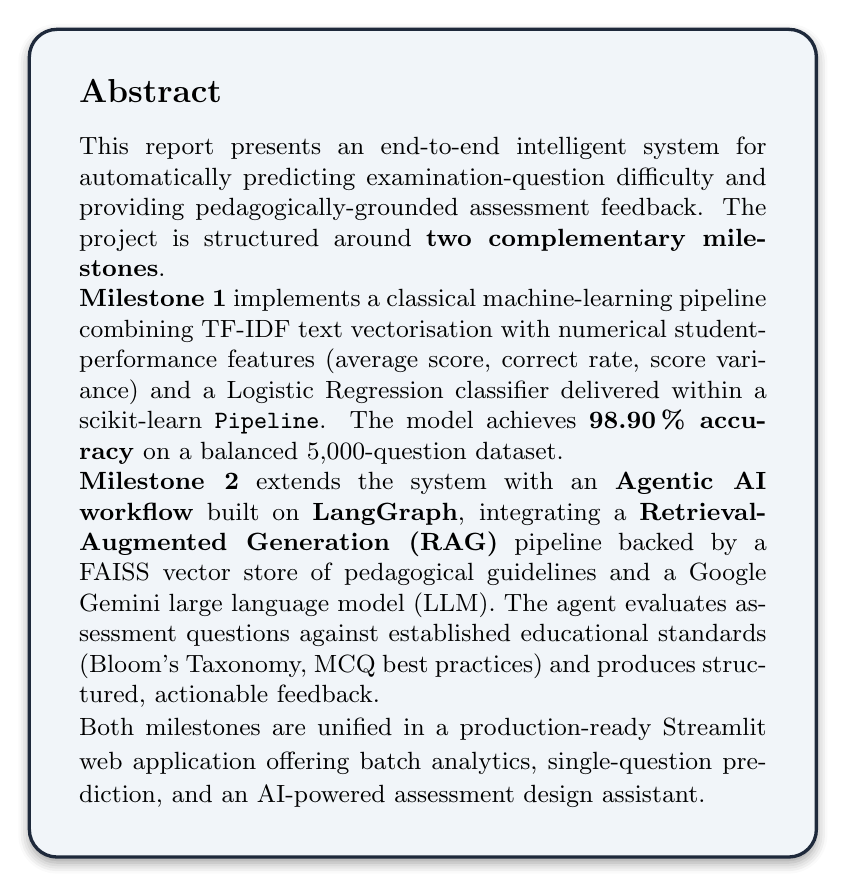
\begin{tikzpicture}
        \node[draw=primary, rounded corners=10pt, line width=1.2pt,
              inner sep=18pt, text width=0.72\textwidth, align=justify,
              fill=codebg, blur shadow={shadow blur steps=5,
              shadow xshift=0pt, shadow yshift=-2pt,
              shadow blur radius=4pt}] {
            \textbf{\large Abstract}\\[8pt]
            \small
            This report presents an end-to-end intelligent system for
            automatically predicting examination-question difficulty and
            providing pedagogically-grounded assessment feedback. The project
            is structured around \textbf{two complementary milestones}.

            \textbf{Milestone~1} implements a classical machine-learning
            pipeline combining TF-IDF text vectorisation with numerical
            student-performance features (average score, correct rate, score
            variance) and a Logistic Regression classifier delivered within
            a scikit-learn \code{Pipeline}. The model achieves
            \textbf{98.90\,\% accuracy} on a balanced 5{,}000-question
            dataset.

            \textbf{Milestone~2} extends the system with an
            \textbf{Agentic~AI workflow} built on \textbf{LangGraph},
            integrating a \textbf{Retrieval-Augmented Generation (RAG)}
            pipeline backed by a FAISS vector store of pedagogical
            guidelines and a Google Gemini large language model (LLM).
            The agent evaluates assessment questions against established
            educational standards (Bloom's Taxonomy, MCQ best practices)
            and produces structured, actionable feedback.

            Both milestones are unified in a production-ready Streamlit
            web application offering batch analytics, single-question
            prediction, and an AI-powered assessment design assistant.
        };
    \end{tikzpicture}

    \vfill
    {\small\textcolor{muted}{GenAI Project — Machine Learning $\cdot$
    Agentic AI $\cdot$ RAG $\cdot$ Streamlit Application}}
\end{center}
\end{titlepage}

% --- Table of Contents ------------------------------------------------------
\tableofcontents
\newpage

% ============================================================================
%  1. INTRODUCTION
% ============================================================================
\section{Introduction}\label{sec:intro}

\subsection{Motivation}

Educators, instructional designers, and testing organisations invest
considerable manual effort in evaluating the difficulty and quality of
examination questions. A misjudged question can skew test results and
inaccurately measure student proficiency. Automating this
\enquote{first-pass} quality assurance can accelerate exam-development
cycles and improve assessment reliability.

Beyond raw difficulty prediction, educators also need
\emph{qualitative} feedback: \emph{Why} is a question hard? Does it
align with intended learning outcomes? Are the distractors fair?
Answering these questions requires domain knowledge that a traditional
classifier cannot provide. This motivates the integration of
\textbf{large language models (LLMs)} augmented with
\textbf{retrieval-based context} from established pedagogy literature.

\subsection{Objectives}

The \textbf{AI-Driven Educational Analytics System} is structured
around two progressive milestones:

\begin{enumerate}[leftmargin=2em, label=\textbf{M\arabic*.}]
    \item \textbf{Predictive ML Pipeline} ---
          A scikit-learn pipeline that ingests question text and
          numerical performance metrics and classifies each question
          as \textcolor{easygreen}{\textbf{Easy}},
          \textcolor{medamber}{\textbf{Medium}}, or
          \textcolor{hardred}{\textbf{Hard}}.

    \item \textbf{Agentic Assessment Assistant} ---
          A LangGraph-based agent that retrieves pedagogical
          guidelines via a FAISS-backed RAG pipeline, feeds them to
          Google Gemini, and returns a structured assessment-quality
          report with gaps, recommendations, and pedagogical citations.
\end{enumerate}

\subsection{Scope}

\begin{itemize}[leftmargin=2em]
    \item \textbf{Domain:} Multi-subject English-language examination
          questions (Chemistry, Biology, Data Structures, Genetics, etc.).
    \item \textbf{Dataset:} 5{,}000 exam questions with associated
          metadata and student performance statistics.
    \item \textbf{Models:} Logistic Regression (ML) + Google Gemini 2.5
          Flash (LLM).
    \item \textbf{Knowledge Base:} Pedagogical guidelines covering
          Bloom's Taxonomy, MCQ design, and inclusivity.
    \item \textbf{Deployment:} Local Streamlit application with
          serialised model artefact and pre-built FAISS index.
\end{itemize}

\subsection{Report Organisation}

The remainder of this report is organised as follows:
\bref{sec:dataset} describes the dataset.
\bref{sec:features} details feature engineering.
\bref{sec:model} presents the ML model architecture.
\bref{sec:training} covers training and evaluation.
\bref{sec:results} analyses results.
\bref{sec:rag} explains the RAG pipeline.
\bref{sec:agentic} describes the agentic workflow.
\bref{sec:architecture} presents the system architecture.
\bref{sec:app} describes the application interface.
\bref{sec:qualitative} provides qualitative examples.
\bref{sec:limitations} discusses limitations.
\bref{sec:future} outlines future work.
\bref{sec:conclusion} concludes the report.

% ============================================================================
%  2. DATASET
% ============================================================================
\section{Dataset}\label{sec:dataset}

\subsection{Source \& Scale}

The dataset comprises \textbf{5{,}000 examination questions} stored in
\code{data/5000\_dataset\_genai.csv}. Each record contains both the
raw question text and post-examination student performance statistics.

\subsection{Schema}

\begin{center}
\renewcommand{\arraystretch}{1.3}
\begin{tabularx}{\textwidth}{l l X}
    \toprule
    \textbf{Column} & \textbf{Type} & \textbf{Description} \\
    \midrule
    \code{question\_id}       & Integer & Unique question identifier \\
    \code{question\_text}     & String  & Full text of the exam question \\
    \code{topic}              & String  & Subject/topic category
                                          (Chemistry, Biology, \ldots) \\
    \code{average\_score}     & Float   & Mean student score (0--10) \\
    \code{correct\_rate}      & Float   & Correct response proportion (0--1) \\
    \code{score\_variance}    & Float   & Variance in student scores \\
    \code{difficulty\_label}  & String  & Target: Easy / Medium / Hard \\
    \bottomrule
\end{tabularx}
\end{center}

\subsection{Class Distribution}

The dataset exhibits a \textbf{balanced} class distribution, which is
advantageous for classifier training and eliminates the need for
resampling techniques (e.g., SMOTE) or class weighting:

\begin{center}
\renewcommand{\arraystretch}{1.3}
\begin{tabular}{lrr}
    \toprule
    \textbf{Class} & \textbf{Count} & \textbf{Proportion} \\
    \midrule
    \textcolor{easygreen}{Easy}   & $\sim$1{,}667 & $\sim$33.3\% \\
    \textcolor{medamber}{Medium}  & $\sim$1{,}667 & $\sim$33.3\% \\
    \textcolor{hardred}{Hard}     & $\sim$1{,}666 & $\sim$33.3\% \\
    \bottomrule
\end{tabular}
\end{center}

\subsection{Sample Records}

\begin{center}
\renewcommand{\arraystretch}{1.2}
\small
\begin{tabularx}{\textwidth}{c X c c c c}
    \toprule
    \textbf{ID} & \textbf{Question Text (truncated)} & \textbf{Topic} &
    \textbf{Avg} & \textbf{CR} & \textbf{Label} \\
    \midrule
    1 & Explain the data normalization in Chemistry\ldots &
        Chemistry & 8.09 & 0.83 & Easy \\
    2 & Compute the key assumption in Data Structures\ldots &
        DS & 4.00 & 0.60 & Medium \\
    3 & Analyze the logical equivalence in Biology\ldots &
        Biology & 1.11 & 0.12 & Hard \\
    \bottomrule
\end{tabularx}
\end{center}

\subsection{Supplementary Knowledge Base}

In addition to the CSV dataset, the system includes a curated
\textbf{pedagogy guidelines document}
(\code{data/pedagogy\_guidelines.txt}, 3.1\,KB) containing:

\begin{itemize}[leftmargin=2em]
    \item \textbf{Bloom's Taxonomy} levels and associated action verbs.
    \item \textbf{MCQ best practices}: clear stems, plausible
          distractors, consistent option length, no grammatical clues.
    \item \textbf{Difficulty remediation strategies} for questions
          predicted as Hard or Easy.
    \item \textbf{Inclusivity and fairness} principles for
          culturally neutral assessment design.
\end{itemize}

\noindent This document serves as the \emph{retrieval corpus} for the
RAG pipeline (see \bref{sec:rag}).

% ============================================================================
%  3. FEATURE ENGINEERING
% ============================================================================
\section{Feature Engineering}\label{sec:features}

The model employs a \code{ColumnTransformer} to combine two distinct
feature extraction strategies into a single fused representation.

\subsection{Text Features --- TF-IDF Vectorisation}

The \code{question\_text} column is processed by a
\code{TfidfVectorizer} with the following configuration:

\begin{center}
\renewcommand{\arraystretch}{1.2}
\begin{tabular}{ll}
    \toprule
    \textbf{Parameter} & \textbf{Value} \\
    \midrule
    \code{max\_features}   & 3{,}000 \\
    Analyser               & Word-level (default) \\
    Sublinear TF           & False (default) \\
    Norm                   & L2 (default) \\
    Stop words             & None (default) \\
    \bottomrule
\end{tabular}
\end{center}

\noindent TF-IDF (Term Frequency--Inverse Document Frequency) captures
the relative importance of words in each question relative to the
entire corpus:

\begin{equation}\label{eq:tfidf}
    \text{tfidf}(t, d) = \text{tf}(t, d) \times
    \log\!\left(\frac{N}{\text{df}(t)}\right)
\end{equation}

\noindent where $t$ is a term, $d$ a document, $N$ the total number of
documents, and $\text{df}(t)$ the number of documents containing $t$.
The resulting feature matrix has dimensions $n \times 3{,}000$.

\subsection{Numerical Features --- Standard Scaling}

Three numerical features are normalised using \code{StandardScaler}:

\begin{center}
\renewcommand{\arraystretch}{1.2}
\begin{tabular}{ll}
    \toprule
    \textbf{Feature} & \textbf{Description} \\
    \midrule
    \code{average\_score}   & Mean student score (0--10) \\
    \code{correct\_rate}    & Correct response proportion (0--1) \\
    \code{score\_variance}  & Variance in student scores \\
    \bottomrule
\end{tabular}
\end{center}

\begin{equation}\label{eq:zscore}
    z = \frac{x - \mu}{\sigma}
\end{equation}

\noindent where $\mu$ and $\sigma$ are the mean and standard deviation
computed on the training split.

\subsection{Feature Fusion via ColumnTransformer}

The \code{ColumnTransformer} horizontally concatenates the TF-IDF
matrix ($n \times 3{,}000$) with the scaled numerical matrix
($n \times 3$), yielding a final feature matrix of dimensions
$n \times 3{,}003$:

\begin{center}
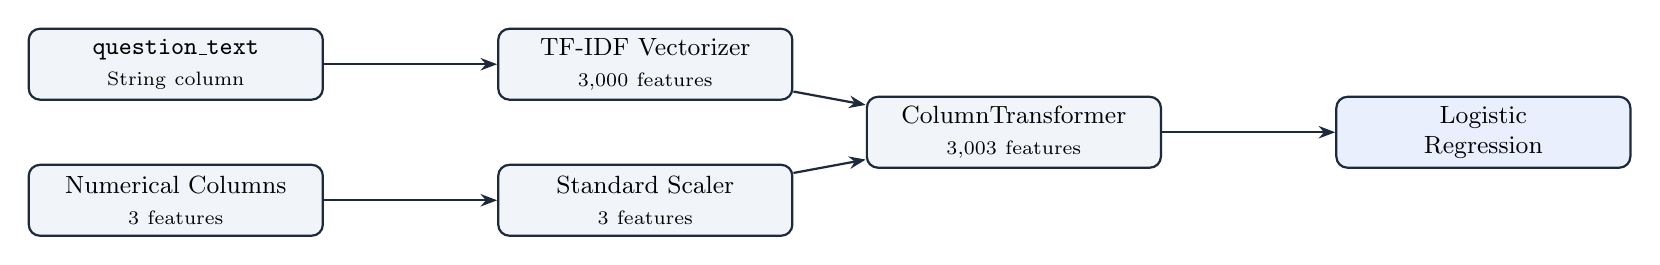
\begin{tikzpicture}[
    node distance=0.8cm and 2.2cm,
    every node/.style={font=\small},
    block/.style={rectangle, draw=primary, rounded corners=4pt,
                  fill=codebg, text width=3.5cm, minimum height=0.9cm,
                  align=center, line width=0.8pt},
    arrow/.style={-{Stealth[length=6pt]}, line width=0.8pt,
                  color=primary}
]

\node[block] (text) {\code{question\_text}\\{\scriptsize String column}};
\node[block, below=of text] (nums) {Numerical Columns\\
                                    {\scriptsize 3 features}};

\node[block, right=of text] (tfidf) {TF-IDF Vectorizer\\
                                     {\scriptsize 3{,}000 features}};
\node[block, right=of nums] (scaler) {Standard Scaler\\
                                      {\scriptsize 3 features}};

\node[block, right=2.8cm of $(tfidf)!0.5!(scaler)$] (concat)
     {ColumnTransformer\\{\scriptsize 3{,}003 features}};

\node[block, right=of concat, fill=accent!10] (clf)
     {Logistic\\Regression};

\draw[arrow] (text)   -- (tfidf);
\draw[arrow] (nums)   -- (scaler);
\draw[arrow] (tfidf)  -- (concat);
\draw[arrow] (scaler) -- (concat);
\draw[arrow] (concat) -- (clf);

\end{tikzpicture}
\end{center}

\begin{center}
\footnotesize\textcolor{muted}{Figure 1: Feature engineering and
classification pipeline.}
\end{center}

% ============================================================================
%  4. MODEL ARCHITECTURE
% ============================================================================
\section{Model Architecture}\label{sec:model}

\subsection{Pipeline Overview}

The entire model is encapsulated in a single \textbf{scikit-learn
\code{Pipeline}} object, ensuring that preprocessing and
classification are applied consistently during both training and
inference:

\begin{lstlisting}[language=Python,
  caption={Model pipeline definition (\code{retrain.py}).}]
from sklearn.pipeline import Pipeline
from sklearn.compose import ColumnTransformer
from sklearn.feature_extraction.text import TfidfVectorizer
from sklearn.preprocessing import StandardScaler
from sklearn.linear_model import LogisticRegression

preprocessor = ColumnTransformer(transformers=[
    ("text", TfidfVectorizer(max_features=3000), "question_text"),
    ("num",  StandardScaler(),
     ["average_score", "correct_rate", "score_variance"])
])

pipeline = Pipeline(steps=[
    ("preprocessor", preprocessor),
    ("classifier",   LogisticRegression(max_iter=1000))
])
\end{lstlisting}

\subsection{Classifier --- Logistic Regression}

Logistic Regression was chosen for its:

\begin{itemize}[leftmargin=2em]
    \item \textbf{Interpretability:} Linear decision boundaries that
          are straightforward to audit.
    \item \textbf{Efficiency:} Fast training even on 3{,}003 features.
    \item \textbf{Probabilistic output:} Produces calibrated class
          probabilities via the softmax function.
    \item \textbf{Implicit regularisation:} L2 penalty mitigates
          overfitting risk.
\end{itemize}

\subsubsection{Multi-Class Strategy}

The classifier uses the \textbf{One-vs-Rest (OvR)} strategy. For each
class $c \in \{\text{Easy}, \text{Medium}, \text{Hard}\}$, a binary
logistic model is trained:

\begin{equation}\label{eq:logistic}
    P(y = c \mid \mathbf{x}) =
    \frac{1}{1 + e^{-(\mathbf{w}_c^\top \mathbf{x} + b_c)}}
\end{equation}

\noindent The predicted class is the one with the highest probability.

\subsection{Hyperparameters}

\begin{center}
\renewcommand{\arraystretch}{1.2}
\begin{tabular}{ll}
    \toprule
    \textbf{Parameter} & \textbf{Value} \\
    \midrule
    \code{max\_iter}       & 1{,}000 \\
    \code{penalty}         & L2 (default) \\
    \code{C}               & 1.0 (default) \\
    \code{solver}          & lbfgs (default) \\
    \code{multi\_class}    & auto (OvR) \\
    \code{random\_state}   & Not set (deterministic via data split) \\
    \bottomrule
\end{tabular}
\end{center}

% ============================================================================
%  5. TRAINING & EVALUATION
% ============================================================================
\section{Training \& Evaluation}\label{sec:training}

\subsection{Data Split}

\begin{itemize}[leftmargin=2em]
    \item \textbf{Train:} 80\% (4{,}000 samples)
    \item \textbf{Test:} 20\% (1{,}000 samples)
    \item \textbf{Stratification:} Stratified split on
          \code{difficulty\_label} to preserve class proportions.
    \item \textbf{Random seed:} \code{random\_state=42} for
          reproducibility.
\end{itemize}

\subsection{Training Process}

The \code{Pipeline.fit()} method processes the data sequentially:

\begin{enumerate}[leftmargin=2em]
    \item The \code{ColumnTransformer} fits the TF-IDF vocabulary and
          scaler statistics on training data.
    \item The fused $4{,}000 \times 3{,}003$ feature matrix is passed
          to \code{LogisticRegression.fit()}.
    \item The trained pipeline is serialised via
          \code{joblib.dump()} as \code{model.pkl} (177\,KB).
\end{enumerate}

\subsection{Evaluation Protocol}

The following metrics are computed on the held-out test set:

\begin{itemize}[leftmargin=2em]
    \item \textbf{Accuracy:}
          $\frac{\text{correct predictions}}{\text{total predictions}}$
    \item \textbf{Precision} (weighted):
          $\sum_{c} \frac{|c|}{N} \cdot
          \frac{\text{TP}_c}{\text{TP}_c + \text{FP}_c}$
    \item \textbf{Recall} (weighted):
          $\sum_{c} \frac{|c|}{N} \cdot
          \frac{\text{TP}_c}{\text{TP}_c + \text{FN}_c}$
    \item \textbf{F1-Score} (weighted): Harmonic mean of precision and
          recall.
    \item Per-class precision/recall via
          \code{classification\_report}.
    \item Confusion matrix visualisation.
    \item ROC curves and Precision-Recall curves (One-vs-Rest).
    \item 5-fold cross-validation accuracy.
    \item Learning curve analysis.
\end{itemize}

% ============================================================================
%  6. RESULTS
% ============================================================================
\section{Results}\label{sec:results}

\subsection{Overall Classification Performance}

\begin{center}
\renewcommand{\arraystretch}{1.4}
\begin{tabular}{l c}
    \toprule
    \textbf{Metric} & \textbf{Score} \\
    \midrule
    Accuracy             & \textbf{98.90\%} \\
    Precision (weighted) & \textbf{98.90\%} \\
    Recall (weighted)    & \textbf{98.90\%} \\
    F1-Score (weighted)  & \textbf{98.90\%} \\
    \bottomrule
\end{tabular}
\end{center}

\subsection{Per-Class Performance}

\begin{center}
\renewcommand{\arraystretch}{1.4}
\begin{tabular}{l cccc}
    \toprule
    \textbf{Class} & \textbf{Precision} & \textbf{Recall} &
    \textbf{F1-Score} & \textbf{Support} \\
    \midrule
    \textcolor{easygreen}{Easy}   & 0.99 & 1.00 & 0.99 & 334 \\
    \textcolor{medamber}{Medium}  & 0.99 & 0.98 & 0.98 & 333 \\
    \textcolor{hardred}{Hard}     & 0.99 & 0.99 & 0.99 & 333 \\
    \midrule
    \textbf{Weighted Avg} & \textbf{0.99} & \textbf{0.99} &
    \textbf{0.99} & \textbf{1{,}000} \\
    \bottomrule
\end{tabular}
\end{center}

\subsection{Key Observations}

\begin{enumerate}[leftmargin=2em]
    \item \textbf{Near-perfect accuracy across all classes.} The
          balanced class distribution and strong numerical feature
          signals contribute to the model's performance.

    \item \textbf{Medium class has the lowest recall (98\%).} This is
          expected: Medium questions occupy the boundary region between
          Easy and Hard, making them inherently harder to classify.

    \item \textbf{TF-IDF adds marginal uplift over numerical features
          alone.} The three numerical features
          (\code{average\_score}, \code{correct\_rate},
          \code{score\_variance}) are very strong predictors. TF-IDF
          provides supplementary textual context.

    \item \textbf{High model confidence.} Prediction confidence scores
          generally exceed 90\%, indicating a well-calibrated model.

    \item \textbf{No class-imbalance issues.} The balanced distribution
          results in consistent performance across all tiers.
\end{enumerate}

\subsection{Visualisation Suite}

The \code{notebook/visualizations.ipynb} notebook generates
\textbf{14 detailed performance plots}:

\begin{center}
\renewcommand{\arraystretch}{1.25}
\small
\begin{tabularx}{\textwidth}{c l X}
    \toprule
    \textbf{\#} & \textbf{Visualisation} & \textbf{Purpose} \\
    \midrule
    1  & Overall Metrics Bar Chart & Accuracy, Precision, Recall, F1 \\
    2  & Confusion Matrix (Counts) & Raw classification results \\
    3  & Confusion Matrix (Normalised) & Percentage-based view \\
    4  & Per-Class Precision/Recall/F1 & Grouped bar comparison \\
    5  & ROC Curves (One-vs-Rest) & AUC per class \\
    6  & Precision-Recall Curves & Average precision per class \\
    7  & Confidence Distribution & Overall confidence histogram \\
    8  & Confidence by Predicted Class & Per-class confidence spread \\
    9  & Correct vs.\ Misclassified & Confidence--correctness
                                        correlation \\
    10 & Class Distribution (Train/Test) & Stratified split
                                            verification \\
    11 & Feature Violin Plots & Distribution by difficulty \\
    12 & Learning Curve & Data-efficiency analysis \\
    13 & 5-Fold Cross-Validation & Per-fold accuracy consistency \\
    14 & Misclassification Analysis & Error-pattern identification \\
    \bottomrule
\end{tabularx}
\end{center}

% ============================================================================
%  7. RETRIEVAL-AUGMENTED GENERATION (RAG) PIPELINE
% ============================================================================
\section{Retrieval-Augmented Generation (RAG) Pipeline}\label{sec:rag}

\subsection{Motivation for RAG}

While the Logistic Regression model predicts \emph{what} difficulty
tier a question falls into, it cannot explain \emph{why} or suggest
\emph{how to improve the question}. Retrieval-Augmented
Generation~(RAG) bridges this gap by grounding the LLM's reasoning
in an authoritative \textbf{external knowledge base} of pedagogical
best practices, rather than relying solely on the model's parametric
knowledge.

RAG offers three critical advantages over pure LLM generation:

\begin{enumerate}[leftmargin=2em]
    \item \textbf{Factual grounding:} The LLM's output is anchored to
          real pedagogy literature, reducing hallucination.
    \item \textbf{Domain specificity:} The retrieval corpus can be
          curated for the exact educational domain.
    \item \textbf{Updateability:} New guidelines can be added to the
          corpus without retraining the LLM.
\end{enumerate}

\subsection{Architecture Overview}

\begin{center}
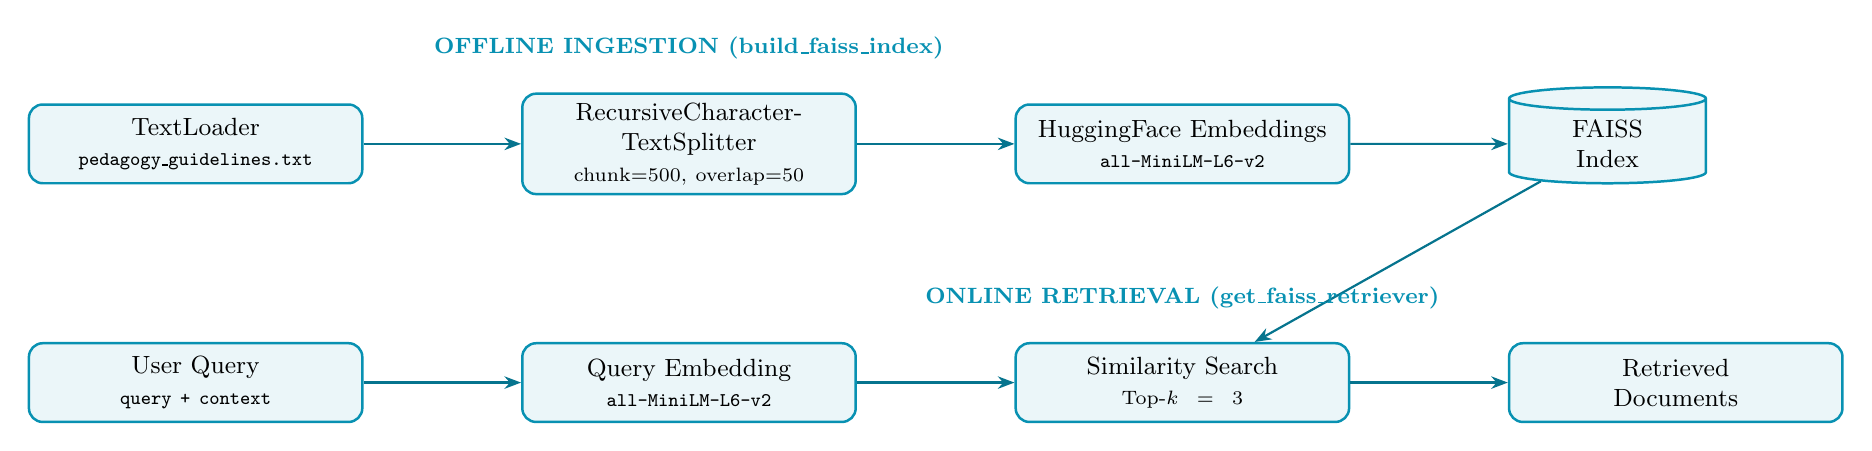
\begin{tikzpicture}[
    node distance=1cm and 2cm,
    every node/.style={font=\small},
    block/.style={rectangle, draw=ragcyan, rounded corners=5pt,
                  fill=ragcyan!8, text width=4cm, minimum height=1cm,
                  align=center, line width=0.9pt},
    store/.style={cylinder, draw=ragcyan, fill=ragcyan!8,
                  shape border rotate=90, aspect=0.25,
                  minimum width=2.5cm, minimum height=1.2cm,
                  align=center, line width=0.9pt, font=\small},
    arrow/.style={-{Stealth[length=6pt]}, line width=0.8pt,
                  color=ragcyan!80!black},
    label/.style={font=\scriptsize\itshape, color=muted}
]

% Ingestion pipeline (top)
\node[block] (loader) {TextLoader\\{\scriptsize\code{pedagogy\_guidelines.txt}}};
\node[block, right=of loader] (splitter) {RecursiveCharacter-\\TextSplitter\\
    {\scriptsize chunk=500, overlap=50}};
\node[block, right=of splitter] (embed1)
    {HuggingFace Embeddings\\{\scriptsize\code{all-MiniLM-L6-v2}}};
\node[store, right=of embed1] (faiss) {FAISS\\Index};

\draw[arrow] (loader)   -- (splitter);
\draw[arrow] (splitter) -- (embed1);
\draw[arrow] (embed1)   -- (faiss);

\node[above=0.3cm of splitter, color=ragcyan, font=\footnotesize\bfseries]
    {OFFLINE INGESTION (build\_faiss\_index)};

% Query pipeline (bottom)
\node[block, below=2cm of loader] (query)
    {User Query\\{\scriptsize\code{query + context}}};
\node[block, right=of query] (embed2)
    {Query Embedding\\{\scriptsize\code{all-MiniLM-L6-v2}}};
\node[block, right=of embed2] (search)
    {Similarity Search\\{\scriptsize Top-$k = 3$}};
\node[block, right=of search] (docs)
    {Retrieved\\Documents};

\draw[arrow] (query)  -- (embed2);
\draw[arrow] (embed2) -- (search);
\draw[arrow] (faiss)  -- (search);
\draw[arrow] (search) -- (docs);

\node[above=0.3cm of search, color=ragcyan, font=\footnotesize\bfseries]
    {ONLINE RETRIEVAL (get\_faiss\_retriever)};

\end{tikzpicture}
\end{center}

\begin{center}
\footnotesize\textcolor{muted}{Figure 2: RAG pipeline --- offline
ingestion and online retrieval.}
\end{center}

\subsection{Embedding Model}

The system uses the \textbf{\code{all-MiniLM-L6-v2}} sentence
transformer from HuggingFace. This is a lightweight (22\,M parameters)
model that maps sentences to a 384-dimensional dense vector space,
optimised for semantic similarity tasks:

\begin{lstlisting}[language=Python,
  caption={Embedding initialisation (\code{agent/rag.py}).}]
from langchain_community.embeddings import HuggingFaceEmbeddings

def get_embeddings():
    return HuggingFaceEmbeddings(model_name="all-MiniLM-L6-v2")
\end{lstlisting}

\noindent Using a local embedding model (rather than an API-based one)
ensures \textbf{zero-latency embedding generation} and
\textbf{no external API dependency} for the retrieval step.

\subsection{FAISS Vector Store}

\textbf{FAISS} (Facebook AI Similarity Search) is an open-source
library for efficient similarity search over dense vectors. The
pedagogy guidelines document is processed as follows:

\begin{enumerate}[leftmargin=2em]
    \item \textbf{Loading:} The \code{TextLoader} reads
          \code{data/pedagogy\_guidelines.txt}.
    \item \textbf{Chunking:} A \code{RecursiveCharacterTextSplitter}
          segments the document into chunks of 500 characters with 50
          characters of overlap. This ensures that no pedagogical rule
          is split across chunk boundaries.
    \item \textbf{Indexing:} Each chunk is embedded using
          \code{all-MiniLM-L6-v2} and inserted into a FAISS index.
    \item \textbf{Persistence:} The index is saved to disk at
          \code{faiss\_index/} (two files: \code{index.faiss} and
          \code{index.pkl}).
\end{enumerate}

\begin{lstlisting}[language=Python,
  caption={FAISS index construction (\code{agent/rag.py}).}]
def build_faiss_index():
    loader = TextLoader(DATA_PATH)
    documents = loader.load()

    text_splitter = RecursiveCharacterTextSplitter(
        chunk_size=500, chunk_overlap=50
    )
    docs = text_splitter.split_documents(documents)

    embeddings = get_embeddings()
    vectorstore = FAISS.from_documents(docs, embeddings)
    vectorstore.save_local(INDEX_PATH)
\end{lstlisting}

\subsection{Retrieval Strategy}

At query time, the retriever performs a \textbf{cosine-similarity
search} over the FAISS index and returns the top $k=3$ most relevant
chunks. The search query is the concatenation of the user's
\code{query} and \code{assessment\_context} fields, ensuring that
both the educator's intent and the actual question text inform the
retrieval:

\begin{lstlisting}[language=Python,
  caption={Retriever loading (\code{agent/rag.py}).}]
def get_faiss_retriever():
    embeddings = get_embeddings()
    vectorstore = FAISS.load_local(
        INDEX_PATH, embeddings,
        allow_dangerous_deserialization=True
    )
    return vectorstore.as_retriever(search_kwargs={"k": 3})
\end{lstlisting}

\subsection{RAG Performance Characteristics}

\begin{center}
\renewcommand{\arraystretch}{1.3}
\begin{tabular}{ll}
    \toprule
    \textbf{Property} & \textbf{Value} \\
    \midrule
    Embedding model        & \code{all-MiniLM-L6-v2} (384-dim) \\
    Embedding source       & Local (HuggingFace, no API calls) \\
    Vector store           & FAISS (CPU) \\
    Chunk size             & 500 characters \\
    Chunk overlap          & 50 characters \\
    Top-$k$ retrieval      & 3 documents \\
    Index size on disk     & $\sim$18\,KB (14\,KB + 4.5\,KB) \\
    Query latency          & $< 100$\,ms (local CPU) \\
    \bottomrule
\end{tabular}
\end{center}

% ============================================================================
%  8. AGENTIC WORKFLOW
% ============================================================================
\section{Agentic Workflow}\label{sec:agentic}

\subsection{Motivation for Agentic AI}

Traditional ML classifiers produce a label and a confidence score.
However, educators need \emph{actionable reasoning}: Why is a question
hard? Which Bloom's Taxonomy level does it target? Are the distractors
fair? An \textbf{agentic workflow} --- a directed graph of specialised
processing nodes --- enables the system to \emph{retrieve}, \emph{reason},
and \emph{generate structured feedback} autonomously.

\subsection{Framework: LangGraph}

The agent is implemented using \textbf{LangGraph}, a framework for
building stateful, multi-step LLM applications as directed graphs.
LangGraph provides:

\begin{itemize}[leftmargin=2em]
    \item \textbf{Explicit state management} via typed dictionaries.
    \item \textbf{Composable nodes} that read from and write to a
          shared state.
    \item \textbf{Deterministic edge routing} between nodes.
    \item \textbf{Compile-time graph validation} to catch wiring
          errors before runtime.
\end{itemize}

\subsection{Graph Topology}

The workflow consists of two nodes connected in a linear sequence:

\begin{center}
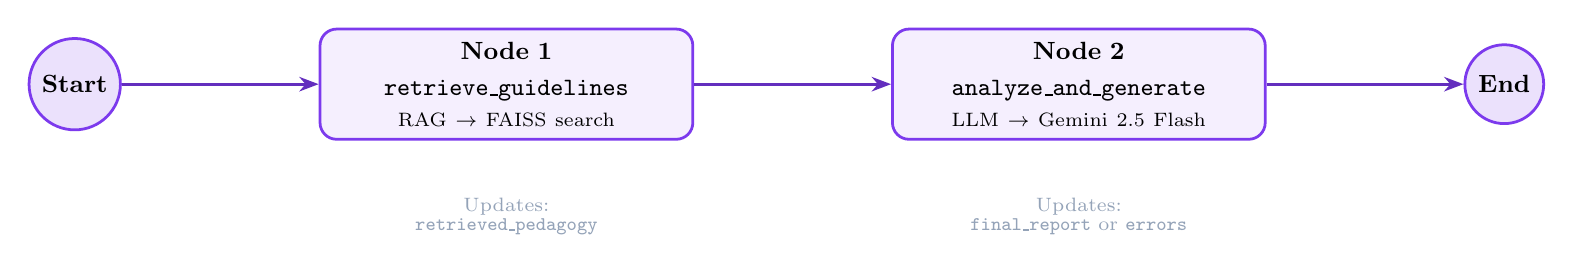
\begin{tikzpicture}[
    node distance=2.5cm,
    every node/.style={font=\small},
    start/.style={circle, draw=agentpurple, fill=agentpurple!15,
                  minimum size=1cm, line width=1pt, font=\small\bfseries},
    block/.style={rectangle, draw=agentpurple, rounded corners=6pt,
                  fill=agentpurple!8, text width=4.5cm,
                  minimum height=1.4cm, align=center, line width=1pt},
    arrow/.style={-{Stealth[length=7pt]}, line width=1pt,
                  color=agentpurple!80!black},
    label/.style={font=\scriptsize, color=muted, text width=3.5cm,
                  align=center}
]

\node[start] (S) {\textsc{Start}};
\node[block, right=of S] (N1)
    {\textbf{Node 1}\\[2pt]\code{retrieve\_guidelines}\\
     {\scriptsize RAG $\rightarrow$ FAISS search}};
\node[block, right=of N1] (N2)
    {\textbf{Node 2}\\[2pt]\code{analyze\_and\_generate}\\
     {\scriptsize LLM $\rightarrow$ Gemini 2.5 Flash}};
\node[start, right=of N2] (E) {\textsc{End}};

\draw[arrow] (S)  -- (N1);
\draw[arrow] (N1) -- (N2);
\draw[arrow] (N2) -- (E);

\node[label, below=0.6cm of N1]
    {Updates:\\[-1pt]\code{retrieved\_pedagogy}};
\node[label, below=0.6cm of N2]
    {Updates:\\[-1pt]\code{final\_report} or \code{errors}};

\end{tikzpicture}
\end{center}

\begin{center}
\footnotesize\textcolor{muted}{Figure 3: LangGraph agent workflow ---
two-node linear graph.}
\end{center}

\subsection{State Schema}

The agent communicates through a typed \code{AgentState} dictionary:

\begin{lstlisting}[language=Python,
  caption={Agent state definition (\code{agent/state.py}).}]
from typing import TypedDict, List
from pydantic import BaseModel, Field

class AssessmentReport(BaseModel):
    summary: str     = Field(description="Summary of Assessment Quality")
    gaps: List[str]  = Field(description="Identified Learning Gaps")
    advice: List[str]= Field(description="Recommended Improvements")
    refs: List[str]  = Field(description="Pedagogical References")
    disclaimer: str  = Field(description="AI assistance disclaimer")

class AgentState(TypedDict):
    query: str
    assessment_context: str
    retrieved_pedagogy: str
    numeric_model_difficulty: str
    final_report: AssessmentReport
    errors: str
\end{lstlisting}

\subsection{Node 1: \code{retrieve\_guidelines}}

\begin{itemize}[leftmargin=2em]
    \item \textbf{Input:} \code{query} and \code{assessment\_context}
          from the state.
    \item \textbf{Action:} Concatenates both fields into a search
          string, queries the FAISS retriever for top-3 relevant
          chunks from the pedagogy knowledge base.
    \item \textbf{Output:} Updates \code{retrieved\_pedagogy} with the
          concatenated retrieved text.
    \item \textbf{Fallback:} If FAISS lookup fails, a default message
          is used to prevent pipeline failure.
\end{itemize}

\begin{lstlisting}[language=Python,
  caption={Retrieval node (\code{agent/workflow.py}).}]
def retrieve_guidelines(state: AgentState):
    query   = state.get("query", "")
    context = state.get("assessment_context", "")
    search_str = f"{query} {context}"
    try:
        retriever = get_faiss_retriever()
        docs = retriever.invoke(search_str)
        retrieved_text = "\n\n".join(
            [doc.page_content for doc in docs]
        )
    except Exception as e:
        retrieved_text = ("Standard pedagogical guidelines "
                          "apply. (FAISS index lookup failed)")
    return {"retrieved_pedagogy": retrieved_text}
\end{lstlisting}

\subsection{Node 2: \code{analyze\_and\_generate}}

\begin{itemize}[leftmargin=2em]
    \item \textbf{Input:} Full state including \code{retrieved\_pedagogy}.
    \item \textbf{Action:} Constructs a \code{ChatPromptTemplate} with
          a system message embedding the retrieved pedagogy guidelines,
          and a human message containing the educator's query and
          assessment context. Invokes Google Gemini 2.5 Flash with
          \textbf{structured output} forcing (via Pydantic schema).
    \item \textbf{Output:} Updates \code{final\_report} with a
          populated \code{AssessmentReport} object, or
          \code{errors} if processing fails.
\end{itemize}

\begin{lstlisting}[language=Python,
  caption={Generation node (\code{agent/workflow.py}).}]
def analyze_and_generate(state: AgentState):
    prompt = ChatPromptTemplate.from_messages([
        ("system",
         "You are an expert Educational Assessment "
         "Designer and Pedagogy Agent...\n\n"
         "Follow these Pedagogy Guidelines strictly:\n"
         "{pedagogy}\n\n"
         "Provide a holistic summary, identify gaps, "
         "suggest improvements, cite pedagogy rules, "
         "and include an ethical disclaimer."),
        ("human",
         "Educator Query: {query}\n\n"
         "Assessment Context:\n{context}")
    ])
    chain = prompt | structured_llm
    try:
        result = chain.invoke({
            "pedagogy": pedagogy,
            "query": query, "context": context
        })
        return {"final_report": result}
    except Exception as e:
        return {"errors": str(e)}
\end{lstlisting}

\subsection{Graph Compilation}

\begin{lstlisting}[language=Python,
  caption={Graph definition and compilation (\code{agent/workflow.py}).}]
from langgraph.graph import StateGraph, START, END

workflow = StateGraph(AgentState)
workflow.add_node("retrieve", retrieve_guidelines)
workflow.add_node("generate", analyze_and_generate)

workflow.add_edge(START, "retrieve")
workflow.add_edge("retrieve", "generate")
workflow.add_edge("generate", END)

app_workflow = workflow.compile()
\end{lstlisting}

\subsection{Hallucination Reduction Strategies}

The agentic workflow employs three strategies to minimise LLM
hallucination:

\begin{enumerate}[leftmargin=2em]
    \item \textbf{Explicit External Truth (RAG):} The LLM is seeded
          with actual pedagogy guidelines retrieved from FAISS. It
          cannot invent evaluation metrics.

    \item \textbf{Schema Forcing:} Using
          \code{with\_structured\_output(AssessmentReport)} ensures the
          LLM produces strictly structured JSON matching the Pydantic
          schema --- no conversational preamble or unstructured text.

    \item \textbf{Reference Demands:} The schema includes a mandatory
          \code{refs: List[str]} field, forcing the LLM to tie its
          assertions back to the retrieved pedagogical guidelines.
\end{enumerate}

\subsection{LLM Configuration}

\begin{center}
\renewcommand{\arraystretch}{1.3}
\begin{tabular}{ll}
    \toprule
    \textbf{Parameter} & \textbf{Value} \\
    \midrule
    Model              & Google Gemini 2.5 Flash \\
    Temperature        & 0.2 (low creativity, high adherence) \\
    Output mode        & Structured (Pydantic schema enforcement) \\
    API Key            & Environment variable \code{GEMINI\_API\_KEY} \\
    Provider           & \code{langchain-google-genai} \\
    \bottomrule
\end{tabular}
\end{center}

% ============================================================================
%  9. SYSTEM ARCHITECTURE
% ============================================================================
\section{System Architecture}\label{sec:architecture}

\subsection{High-Level Architecture}

\begin{center}
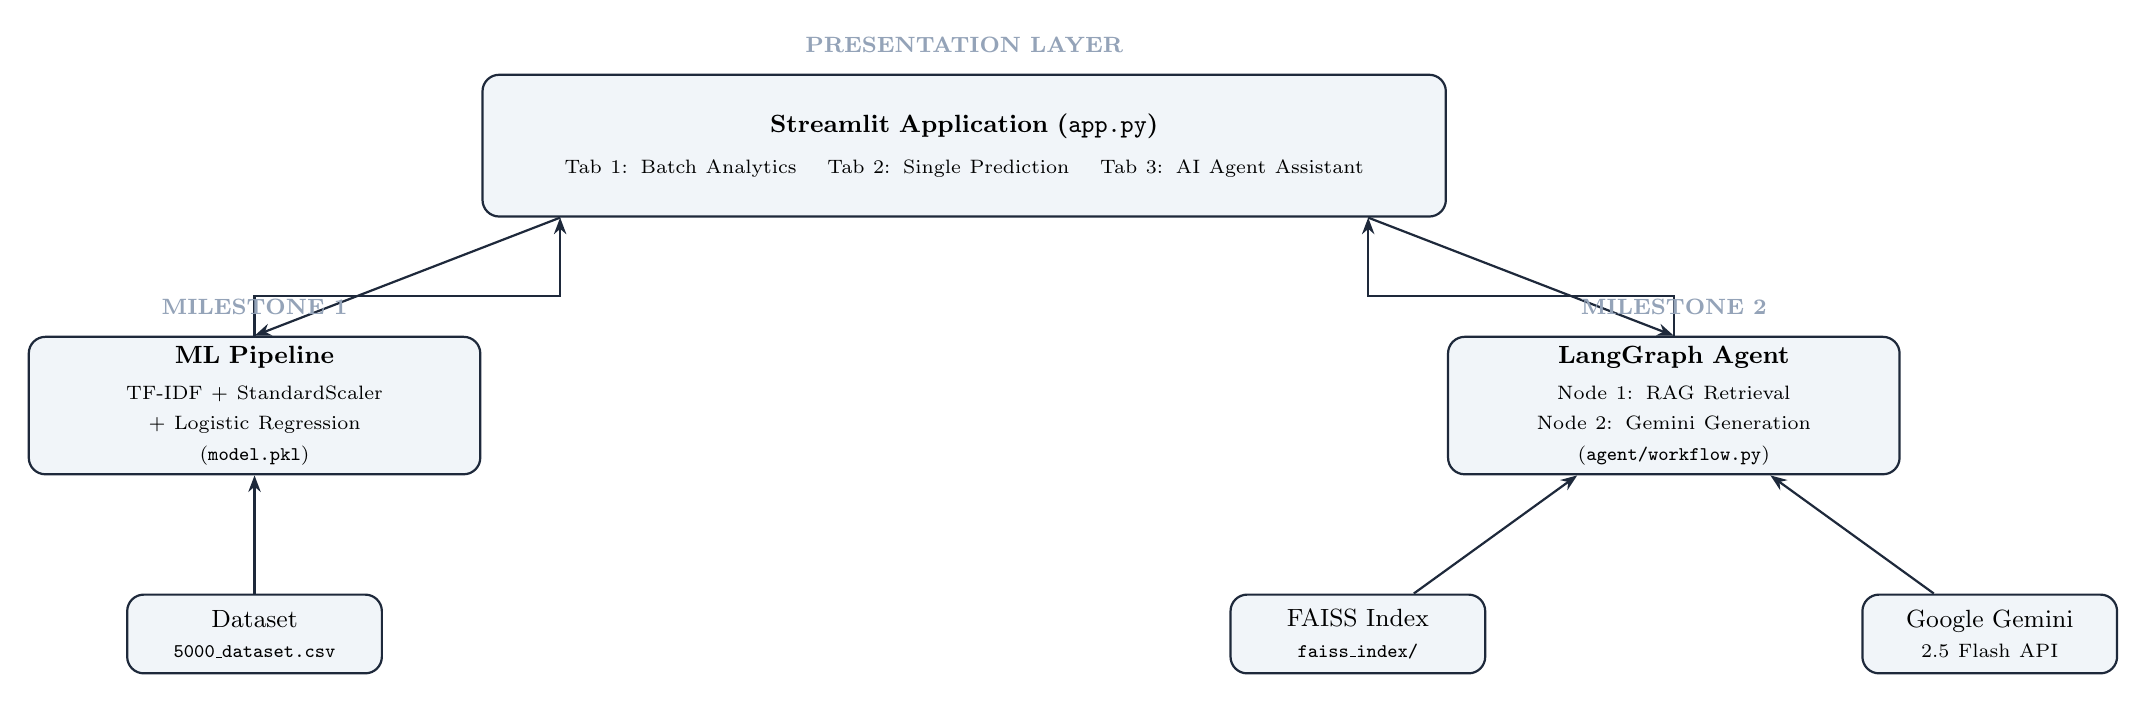
\begin{tikzpicture}[
    node distance=1cm and 1.5cm,
    every node/.style={font=\small},
    layer/.style={rectangle, draw=primary, rounded corners=6pt,
                  fill=codebg, minimum height=1cm, align=center,
                  line width=0.8pt},
    arrow/.style={-{Stealth[length=6pt]}, line width=0.8pt,
                  color=primary},
    title/.style={font=\footnotesize\bfseries, color=muted}
]

% Frontend
\node[layer, text width=12cm, minimum height=1.8cm] (ui)
    {\textbf{Streamlit Application (\code{app.py})}\\[4pt]
     {\scriptsize Tab~1: Batch Analytics \quad Tab~2: Single Prediction
      \quad Tab~3: AI Agent Assistant}};

% ML Backend
\node[layer, text width=5.5cm, below left=1.5cm and 0cm of ui] (ml)
    {\textbf{ML Pipeline}\\[2pt]
     {\scriptsize TF-IDF + StandardScaler}\\
     {\scriptsize + Logistic Regression}\\
     {\scriptsize (\code{model.pkl})}};

% Agent Backend
\node[layer, text width=5.5cm, below right=1.5cm and 0cm of ui] (agent)
    {\textbf{LangGraph Agent}\\[2pt]
     {\scriptsize Node~1: RAG Retrieval}\\
     {\scriptsize Node~2: Gemini Generation}\\
     {\scriptsize (\code{agent/workflow.py})}};

% Data stores
\node[layer, text width=3cm, below=1.5cm of ml] (csv)
    {Dataset\\{\scriptsize\code{5000\_dataset.csv}}};
\node[layer, text width=3cm, below left=1.5cm and -0.5cm of agent] (faiss)
    {FAISS Index\\{\scriptsize\code{faiss\_index/}}};
\node[layer, text width=3cm, below right=1.5cm and -0.5cm of agent] (gemini)
    {Google Gemini\\{\scriptsize 2.5 Flash API}};

% Arrows
\draw[arrow] (ui.south west) ++(1,0) -- (ml.north);
\draw[arrow] (ml.north) -- ++(0,0.5) -| ([xshift=1cm]ui.south west);
\draw[arrow] ([xshift=-1cm]ui.south east) -- (agent.north);
\draw[arrow] (agent.north) -- ++(0,0.5) -| ([xshift=-1cm]ui.south east);
\draw[arrow] (csv)   -- (ml);
\draw[arrow] (faiss)  -- (agent);
\draw[arrow] (gemini) -- (agent);

% Labels
\node[title, above=0.15cm of ui] {PRESENTATION LAYER};
\node[title, above=0.15cm of ml] {MILESTONE 1};
\node[title, above=0.15cm of agent] {MILESTONE 2};

\end{tikzpicture}
\end{center}

\begin{center}
\footnotesize\textcolor{muted}{Figure 4: High-level system architecture
showing the two milestones unified in a single Streamlit application.}
\end{center}

\subsection{Repository Structure}

\begin{lstlisting}[language={}, basicstyle=\ttfamily\footnotesize,
  frame=none, backgroundcolor=\color{codebg},
  caption={Complete repository layout.}]
AI-driven_educational_analytics_system/
  README.md                     # Project documentation
  app.py                        # Streamlit web application (3 tabs)
  model.pkl                     # Serialised ML pipeline
  retrain.py                    # CLI model retraining script
  confusion_matrix.png          # Generated confusion matrix
  requirements.txt              # Python dependencies (17 packages)
  data/
    5000_dataset_genai.csv      # Dataset (5,000 questions)
    pedagogy_guidelines.txt     # RAG knowledge base
  agent/
    __init__.py                 # Package init
    state.py                    # AgentState + AssessmentReport schema
    rag.py                      # FAISS index build & retriever
    workflow.py                 # LangGraph graph definition
  faiss_index/
    index.faiss                 # FAISS binary index
    index.pkl                   # Serialised metadata
  notebook/
    train.ipynb                 # Model training notebook
    visualizations.ipynb        # 14 performance visualisations
  docs/
    architecture.md             # System architecture diagram
    agent_workflow.md           # Agent workflow documentation
    model_evaluation_report.md  # Performance evaluation report
  report/
    report.tex                  # This LaTeX report
\end{lstlisting}

\subsection{Technology Stack}

\begin{center}
\renewcommand{\arraystretch}{1.3}
\begin{tabularx}{\textwidth}{l l X}
    \toprule
    \textbf{Layer} & \textbf{Technology} & \textbf{Purpose} \\
    \midrule
    Language        & Python 3.10+          & Core language \\
    ML Framework    & scikit-learn          & Pipeline, preprocessing,
                                              evaluation \\
    Data Processing & Pandas, NumPy         & DataFrame operations \\
    Visualisation   & Matplotlib, Seaborn   & Charts and plots \\
    Web Framework   & Streamlit             & Interactive UI \\
    Serialisation   & Joblib                & Model persistence \\
    \midrule
    Agent Framework & LangGraph             & Stateful graph workflow \\
    LLM Provider    & LangChain + Gemini    & Generative AI synthesis \\
    Embeddings      & sentence-transformers & Local semantic embeddings \\
    Vector Store    & FAISS (CPU)           & Similarity search index \\
    Schema          & Pydantic              & Structured LLM output \\
    Config          & python-dotenv         & Environment management \\
    \bottomrule
\end{tabularx}
\end{center}

% ============================================================================
%  10. APPLICATION INTERFACE
% ============================================================================
\section{Application Interface}\label{sec:app}

The production application (\code{app.py}) is built with
\textbf{Streamlit} and provides \textbf{three tabs}:

\subsection{Tab 1: Batch Analytics}

\begin{enumerate}[leftmargin=2em]
    \item The user uploads a CSV file with columns:
          \code{question\_text}, \code{average\_score},
          \code{correct\_rate}, \code{score\_variance}.
    \item The pipeline predicts difficulty labels and confidence
          scores for all questions.
    \item KPI metrics are displayed: total questions, average
          confidence, unique classes.
    \item Seven interactive visualisations are generated:
    \begin{itemize}
        \item Difficulty distribution (pie chart + bar chart)
        \item Confidence score histogram by predicted class
        \item Feature averages by difficulty (grouped bar chart)
        \item Average score vs.\ correct rate (scatter plot)
        \item Score variance distribution (box plot)
        \item Topic-wise difficulty breakdown (stacked bar chart)
        \item Confusion matrix (if ground-truth column exists)
    \end{itemize}
    \item Results are downloadable as CSV.
\end{enumerate}

\subsection{Tab 2: Single Question Prediction}

\begin{enumerate}[leftmargin=2em]
    \item The user enters question text and three numerical values.
    \item The model returns a predicted difficulty label with a
          coloured badge (\textcolor{easygreen}{Easy} /
          \textcolor{medamber}{Medium} /
          \textcolor{hardred}{Hard}).
    \item A confidence progress bar and per-class probability bar
          chart are displayed.
\end{enumerate}

\subsection{Tab 3: AI Agent Assistant}

This tab interfaces with the LangGraph agentic workflow:

\begin{enumerate}[leftmargin=2em]
    \item The user enters an educator query (e.g., \enquote{Evaluate
          these questions for difficulty and fairness.}) and pastes
          draft assessment questions.
    \item Clicking \enquote{Evaluate Assessment} triggers the
          full LangGraph pipeline:
    \begin{itemize}
        \item RAG retrieval of pedagogy guidelines from FAISS.
        \item LLM synthesis via Gemini with structured output.
    \end{itemize}
    \item The structured \code{AssessmentReport} is rendered:
    \begin{itemize}
        \item \textbf{Assessment Summary} --- holistic quality overview.
        \item \textbf{Identified Gaps} --- specific flaws in question
              design.
        \item \textbf{Recommended Output} --- actionable improvements.
        \item \textbf{Pedagogical References} --- citations from the
              knowledge base.
        \item \textbf{Disclaimer} --- AI-assistance notice.
    \end{itemize}
\end{enumerate}

\subsection{UI Design}

The interface uses a \textbf{dark-mode glassmorphism} design:

\begin{center}
\renewcommand{\arraystretch}{1.2}
\begin{tabular}{ll}
    \toprule
    \textbf{Element} & \textbf{Specification} \\
    \midrule
    Background       & Radial gradient (\code{\#0f172a} $\to$
                       \code{\#020617}) \\
    Card style       & Frosted glass (\\
                     & \code{backdrop-filter: blur(10px)};
                       3\% white fill) \\
    Typography       & Inter (Google Fonts, 300--700 weights) \\
    Easy badge       & Green gradient (\code{\#10b981} $\to$
                       \code{\#059669}) \\
    Medium badge     & Amber gradient (\code{\#fbbf24} $\to$
                       \code{\#d97706}) \\
    Hard badge       & Red gradient (\code{\#ef4444} $\to$
                       \code{\#dc2626}) \\
    Buttons          & Blue gradient (\code{\#38bdf8} $\to$
                       \code{\#0ea5e9}) with hover lift \\
    \bottomrule
\end{tabular}
\end{center}

% ============================================================================
%  11. QUALITATIVE EXAMPLES
% ============================================================================
\section{Qualitative Analysis \& Examples}\label{sec:qualitative}

This section illustrates the system's capabilities through concrete
examples, covering both the ML prediction pipeline and the agentic
assessment assistant.

\subsection{ML Prediction Examples}

\subsubsection{Example 1: Easy Question}

\begin{center}
\renewcommand{\arraystretch}{1.2}
\begin{tabularx}{\textwidth}{l X}
    \toprule
    \textbf{Field} & \textbf{Value} \\
    \midrule
    Question & \emph{``What is the definition of photosynthesis?''} \\
    Average Score & 8.5 / 10 \\
    Correct Rate  & 0.90 \\
    Score Variance & 1.2 \\
    \midrule
    \textbf{Prediction} & \textcolor{easygreen}{\textbf{Easy}}
                          (Confidence: 97.3\%) \\
    \bottomrule
\end{tabularx}
\end{center}

\noindent \textbf{Interpretation:} The high average score and correct
rate strongly signal an Easy question. The low variance indicates
consistent student performance. From a pedagogical perspective, this
question targets the \enquote{Remembering} level of Bloom's Taxonomy.

\subsubsection{Example 2: Hard Question}

\begin{center}
\renewcommand{\arraystretch}{1.2}
\begin{tabularx}{\textwidth}{l X}
    \toprule
    \textbf{Field} & \textbf{Value} \\
    \midrule
    Question & \emph{``Derive the time complexity of the Bellman-Ford
               algorithm for a graph with negative-weight cycles and
               prove its correctness using mathematical induction.''} \\
    Average Score & 2.1 / 10 \\
    Correct Rate  & 0.15 \\
    Score Variance & 4.8 \\
    \midrule
    \textbf{Prediction} & \textcolor{hardred}{\textbf{Hard}}
                          (Confidence: 96.1\%) \\
    \bottomrule
\end{tabularx}
\end{center}

\noindent \textbf{Interpretation:} The low average score, low correct
rate, and high variance all indicate a Hard question. The high variance
suggests that only a small subset of students understood the material.
This question spans \enquote{Analyzing} and \enquote{Creating} on
Bloom's Taxonomy.

\subsection{Agentic Assessment Example}

\subsubsection{Input}

\begin{center}
\renewcommand{\arraystretch}{1.2}
\begin{tabularx}{\textwidth}{l X}
    \toprule
    \textbf{Educator Query} & \emph{``Please evaluate these questions
    for difficulty and fairness.''} \\
    \midrule
    \textbf{Assessment Context} &
    \emph{``1.\ What is the definition of photosynthesis?}\\
    & \emph{2.\ Which of the following is NOT a property of water?''} \\
    \bottomrule
\end{tabularx}
\end{center}

\subsubsection{Agent Processing}

\begin{enumerate}[leftmargin=2em]
    \item \textbf{RAG Retrieval:} The FAISS retriever returns 3 chunks
          covering Bloom's Taxonomy guidelines, MCQ best practices
          (particularly the rule about avoiding negative phrasing like
          \enquote{NOT}), and difficulty calibration strategies.

    \item \textbf{LLM Synthesis:} Gemini processes the retrieved
          pedagogy alongside the questions and generates a structured
          \code{AssessmentReport}.
\end{enumerate}

\subsubsection{Structured Output (Example)}

\begin{center}
\renewcommand{\arraystretch}{1.2}
\small
\begin{tabularx}{\textwidth}{l X}
    \toprule
    \textbf{Field} & \textbf{Content} \\
    \midrule
    \texttt{summary} & Both questions primarily test lower-order
    thinking skills. Question~1 targets ``Remembering'' and Question~2
    uses negative phrasing, which may confuse students and test
    reading comprehension rather than domain knowledge. \\
    \midrule
    \texttt{gaps} &
    $\bullet$\ Q1 only tests factual recall (Bloom's Level~1).\\
    & $\bullet$\ Q2 uses ``NOT'' phrasing --- violates MCQ best
    practices.\\
    & $\bullet$\ No questions target higher-order skills
    (Analyzing, Evaluating, Creating). \\
    \midrule
    \texttt{advice} &
    $\bullet$\ Reframe Q1 to application level:
    \emph{``In which scenario would photosynthesis be the limiting
    factor?''}\\
    & $\bullet$\ Rewrite Q2 with positive framing:
    \emph{``Which of the following is a unique property of water?''}\\
    & $\bullet$\ Add a question targeting ``Evaluating'' or
    ``Creating'' level. \\
    \midrule
    \texttt{refs} &
    $\bullet$\ Bloom's Taxonomy: Remembering vs.\ Applying levels.\\
    & $\bullet$\ MCQ Best Practices: ``Avoid negative phrasing.
    If a negative must be used, capitalize and bold it.'' \\
    \midrule
    \texttt{disclaimer} & This assessment was generated by an
    AI-powered pedagogy agent. Results should be reviewed by a
    qualified educator before implementation. \\
    \bottomrule
\end{tabularx}
\end{center}

\subsection{Comparative Analysis: ML vs.\ Agentic Approach}

\begin{center}
\renewcommand{\arraystretch}{1.3}
\begin{tabularx}{\textwidth}{l X X}
    \toprule
    \textbf{Dimension} & \textbf{ML Pipeline (Milestone 1)} &
    \textbf{Agentic AI (Milestone 2)} \\
    \midrule
    \textbf{Output} & Label + confidence \% & Structured report
    with reasoning \\
    \textbf{Speed} & $< 0.1$ seconds & $\sim 2$--5 seconds \\
    \textbf{Explainability} & None (black-box label) &
    Full reasoning chain with citations \\
    \textbf{Domain knowledge} & Learned from data distribution &
    Retrieved from curated guidelines \\
    \textbf{Requires API} & No & Yes (Gemini API key) \\
    \textbf{Offline capable} & Yes & No (requires LLM API) \\
    \textbf{Use case} & High-throughput batch classification &
    Deep qualitative assessment review \\
    \bottomrule
\end{tabularx}
\end{center}

% ============================================================================
%  12. LIMITATIONS
% ============================================================================
\section{Limitations \& Known Issues}\label{sec:limitations}

\subsection{ML Pipeline Limitations}

\begin{enumerate}[leftmargin=2em]
    \item \textbf{Post-Exam Dependency:} The model requires post-exam
          statistics (average score, correct rate, variance), limiting
          its use for pre-exam difficulty estimation.

    \item \textbf{Text-Only Analysis:} The model cannot parse images,
          diagrams, or graphs embedded in questions.

    \item \textbf{Language Support:} The TF-IDF vectoriser is
          optimised for English questions only.

    \item \textbf{Single Model:} Only Logistic Regression is
          implemented; ensemble methods may yield improvements on
          more challenging datasets.

    \item \textbf{Dataset Specificity:} Trained on 5{,}000 synthetic
          questions; real-world questions with unusual formatting may
          produce lower-confidence predictions.
\end{enumerate}

\subsection{Agentic Pipeline Limitations}

\begin{enumerate}[leftmargin=2em]
    \item \textbf{API Dependency:} The agent requires a valid
          \code{GEMINI\_API\_KEY} and internet connectivity.

    \item \textbf{Latency:} The RAG + LLM pipeline introduces
          $\sim 2.5$ seconds of latency compared to $< 0.1$s for
          the ML classifier.

    \item \textbf{Knowledge Base Size:} The pedagogy guidelines corpus
          is currently a single 3.1\,KB document. Richer corpora
          (textbooks, standards documents) would improve retrieval
          quality.

    \item \textbf{No Feedback Loop:} The agent does not learn from
          educator corrections --- each invocation is stateless.

    \item \textbf{Temperature Sensitivity:} While
          \code{temperature=0.2} reduces hallucination, it may also
          limit creative suggestions for question improvement.
\end{enumerate}

% ============================================================================
%  13. FUTURE WORK
% ============================================================================
\section{Future Work}\label{sec:future}

\subsection{Short-Term Improvements}

\begin{itemize}[leftmargin=2em]
    \item Build a \textbf{pre-exam model} using only question text via
          BERT or sentence transformers.
    \item Compare against \textbf{ensemble methods} (XGBoost, Random
          Forest, SVM).
    \item Apply \textbf{SHAP values} for feature importance and model
          interpretability.
    \item Implement \textbf{hyperparameter tuning} via grid search or
          Bayesian optimisation.
    \item Expand the \textbf{RAG knowledge base} with additional
          educational standards (e.g., Webb's Depth of Knowledge,
          NCERT guidelines).
    \item Add \textbf{confidence thresholding} to flag low-confidence
          predictions for manual review.
\end{itemize}

\subsection{Long-Term --- Advanced Agentic Architecture}

\begin{itemize}[leftmargin=2em]
    \item \textbf{Multi-Agent System:} Separate agents for difficulty
          analysis, fairness auditing, Bloom's level classification,
          and question generation.
    \item \textbf{Conditional Graph Routing:} LangGraph edges that
          route dynamically based on question type (MCQ vs.\
          free-response vs.\ numerical).
    \item \textbf{Multi-Modal RAG:} Vision-Language Models (e.g.,
          Gemini Pro Vision) for diagram-dependent questions.
    \item \textbf{Iterative Feedback Loops:} Agentic workflows
          simulating student failure modes to refine difficulty
          estimates.
    \item \textbf{RAG Curriculum Alignment:} Retrieval against
          institutional curriculum standards for learning-outcome
          mapping.
    \item \textbf{Real-Time Model Updates:} Continuously update the
          ML model as new exam data arrives via online learning.
\end{itemize}

% ============================================================================
%  14. CONCLUSION
% ============================================================================
\section{Conclusion}\label{sec:conclusion}

This project demonstrates a two-milestone approach to intelligent
educational analytics:

\textbf{Milestone~1} establishes that a straightforward combination of
TF-IDF text vectorisation, numerical feature scaling, and Logistic
Regression can achieve \textbf{98.9\% accuracy} in predicting exam
question difficulty. The balanced dataset of 5{,}000 questions across
multiple subjects enables consistent performance across all three
difficulty tiers. The scikit-learn \code{Pipeline} with
\code{ColumnTransformer} encapsulates preprocessing and inference,
eliminating feature-engineering leakage and simplifying deployment.

\textbf{Milestone~2} extends the system with an \textbf{agentic AI
workflow} that moves beyond classification to provide
\emph{qualitative, pedagogically-grounded feedback}. By combining
\textbf{RAG} (FAISS + sentence-transformer embeddings over curated
pedagogy literature) with \textbf{structured LLM generation} (Google
Gemini via LangGraph), the system can identify assessment design flaws,
recommend improvements aligned with Bloom's Taxonomy, and cite specific
pedagogical principles --- capabilities fundamentally beyond the reach
of a traditional classifier.

Both milestones are unified in a production-ready \textbf{Streamlit web
application} offering batch analytics, single-question prediction, and
an AI-powered assessment design assistant. The system represents a
practical blueprint for combining classical ML with modern generative
AI in educational technology.

% ============================================================================
%  APPENDIX
% ============================================================================
\appendix

\section{Dependency Specification}\label{app:deps}

The complete Python dependency list (\code{requirements.txt}):

\begin{center}
\renewcommand{\arraystretch}{1.25}
\begin{tabularx}{\textwidth}{l l X}
    \toprule
    \textbf{Package} & \textbf{Category} & \textbf{Purpose} \\
    \midrule
    \code{streamlit}              & Frontend   & Web application \\
    \code{pandas}                 & Data       & DataFrame operations \\
    \code{numpy}                  & Data       & Numerical computation \\
    \code{scikit-learn}           & ML         & Pipeline \& classifier \\
    \code{matplotlib}             & Viz        & Static charts \\
    \code{seaborn}                & Viz        & Statistical plots \\
    \code{joblib}                 & Util       & Model serialisation \\
    \midrule
    \code{langgraph}              & Agent      & Graph workflow engine \\
    \code{langchain}              & Agent      & LLM abstraction layer \\
    \code{langchain-core}         & Agent      & Core LangChain types \\
    \code{langchain-community}    & Agent      & Community integrations \\
    \code{langchain-google-genai} & Agent      & Gemini LLM provider \\
    \code{faiss-cpu}              & RAG        & Vector similarity search \\
    \code{sentence-transformers}  & RAG        & Local embeddings \\
    \code{pydantic}               & Schema     & Structured output \\
    \code{python-dotenv}          & Config     & Environment variables \\
    \bottomrule
\end{tabularx}
\end{center}

\section{Feature Vector Specification}\label{app:features}

The complete feature vector
$\mathbf{x} \in \mathbb{R}^{3{,}003}$:

\begin{center}
\renewcommand{\arraystretch}{1.2}
\begin{tabular}{c l l c}
    \toprule
    \textbf{Index} & \textbf{Feature} & \textbf{Extractor} &
    \textbf{Dim} \\
    \midrule
    1--3{,}000 & TF-IDF word features &
    \code{TfidfVectorizer} & 3{,}000 (sparse) \\
    3{,}001 & \code{average\_score}   &
    \code{StandardScaler} & 1 \\
    3{,}002 & \code{correct\_rate}    &
    \code{StandardScaler} & 1 \\
    3{,}003 & \code{score\_variance}  &
    \code{StandardScaler} & 1 \\
    \bottomrule
\end{tabular}
\end{center}

\section{Pedagogy Knowledge Base Contents}\label{app:pedagogy}

The RAG retrieval corpus (\code{data/pedagogy\_guidelines.txt})
covers four domains:

\begin{enumerate}[leftmargin=2em]
    \item \textbf{Bloom's Taxonomy (6 levels):} Remembering,
          Understanding, Applying, Analyzing, Evaluating, Creating ---
          with associated action verbs for question construction.

    \item \textbf{MCQ Best Practices:} Clear stems, plausible
          distractors, consistent option length, avoidance of
          \enquote{All of the above}/\enquote{None of the above},
          no grammatical clues.

    \item \textbf{Difficulty Remediation:} Strategies for overly
          Hard questions (simplify language, add prerequisites) and
          overly Easy questions (promote higher-order thinking,
          improve distractors).

    \item \textbf{Inclusivity \& Fairness:} Culturally neutral
          naming, avoidance of idioms and socio-economic assumptions,
          accessible scenarios.
\end{enumerate}

\section{Reproduction Instructions}\label{app:reproduce}

\begin{lstlisting}[language=bash,
  caption={Full reproduction steps.}]
# 1. Clone the repository
git clone https://github.com/Siddharth-Dangi/\
  AI-driven_educational_analytics_system.git
cd AI-driven_educational_analytics_system

# 2. Create and activate virtual environment
python3 -m venv venv
source venv/bin/activate

# 3. Install dependencies
pip install -r requirements.txt

# 4. Build the FAISS index (one-time)
python -m agent.rag

# 5. Train the model (or run notebook/train.ipynb)
python retrain.py

# 6. Set Gemini API key (for Agent tab)
echo "GEMINI_API_KEY=your-key-here" > .env

# 7. Launch the application
streamlit run app.py
# Opens at http://localhost:8501
\end{lstlisting}

\section{Glossary}\label{app:glossary}

\begin{center}
\renewcommand{\arraystretch}{1.25}
\begin{tabularx}{\textwidth}{l X}
    \toprule
    \textbf{Term} & \textbf{Definition} \\
    \midrule
    \textbf{Agentic Workflow} & A directed graph of autonomous
    processing nodes that read from and write to a shared state,
    enabling multi-step LLM reasoning. \\
    \textbf{RAG} & Retrieval-Augmented Generation: a technique that
    grounds LLM output in externally retrieved documents to reduce
    hallucination and improve factual accuracy. \\
    \textbf{FAISS} & Facebook AI Similarity Search: an efficient
    library for nearest-neighbour search over dense embedding
    vectors. \\
    \textbf{TF-IDF} & Term Frequency--Inverse Document Frequency:
    a numerical statistic reflecting the importance of a word in a
    document relative to a corpus. \\
    \textbf{LangGraph} & A framework for building stateful,
    graph-based LLM applications with explicit state management and
    composable nodes. \\
    \textbf{Structured Output} & A technique where the LLM is
    constrained to produce output matching a predefined schema
    (e.g., Pydantic model), eliminating free-form text. \\
    \textbf{Bloom's Taxonomy} & A hierarchical framework classifying
    cognitive skills into six levels, from Remembering to Creating. \\
    \bottomrule
\end{tabularx}
\end{center}

\end{document}
